\section{Data Simulation}\label{sec:dataset}
To test the performance of the algorithm, simulated data, corresponding to the model $\mathbf{Y} = \mathbf{A}\mathbf{X}$, is needed. All data sets are simulated based on the following approach, satisfying the sufficient conditions for recovery, displayed in theorem \ref{th:conditions}.
 
A source matrix $\mathbf{X} \in \mathbb{R}^{N \times L}$ is constructed, such that a non-zero row is sampled independently of each non-zeros rows over $L$ samples or a zero row. 
By the sources being independent and having zero mean the rows of $\mathbf{X}$ become close to orthogonal \cite{Balkan2014},
%As such the non-zero rows of $\mathbf{X}$ are mutually orthogonal\todo{Kan ikke finde noget på at independent rows af matrix leder til at den også er ortgonal. En matrix er ortogonal hvis $X * X^T = I$ eller $X^T = X^{-1}$}
which approximate the first conditions of theorem \ref{th:conditions}.   
Then a mixing matrix $\mathbf{A} \in \mathbb{R}^{M \times N}$ is constructed with identically distributed and independent entries. 
As such the source signals are randomly mixed and the mixing matrix fulfils the second condition of theorem \ref{th:conditions}.
With known $\mathbf{A}$ and $\mathbf{X}$ the measurement matrix $\mathbf{Y} \in \mathbb{R}^{M \times L}$ is simulated according to the model, by the matrix product $\mathbf{Y} = \mathbf{AX}$. Note that the error matrix $\mathbf{E}$ is omitted in this chapter, as noise is not included in the synthetic data.  

Two different kinds of data sets are simulated.
One deterministic data set with simple and predictable source signals to ensure a solution and easy visualization.
And a stochastic data set with randomized and fluctuating source signals to resemble realistic EEG measurements.

\subsection{Deterministic Data Set}\label{subseg_simpledata}
Two different deterministic data sets are simulated, with a different number of zero rows. 
The first is specified by $N = 5$, $k = 4$, $M = 3$ and $L = 1000$. That is a source matrix $\mathbf{X}$ with $4$ rows generated independently and $1$ zero row which is mixed into a measurement matrix with $3$ measurement per sample.  
The second deterministic data set is specified by $N = 8$, $k = 4$, $M = 3$ and $L = 1000$. This is 3 additional zero rows.
From the specifications the first data set comply to $N \leq \frac{M(M+1)}{2}$ which imply the use of Cov-DL2.
The second data set comply to $N > \frac{M(M+1)}{2}$ and $k \leq \frac{M(M+1)}{2}$ implying the use of Cov-DL1. 
As such it is possible to test both branches of the Cov-DL algorithm. 
     
The four different source signals of $\mathbf{X}$ are defined to be approximately orthogonal by
\begin{itemize}
\item[1.] a sinus signal $\sin(2t)$
\item[2.] a sawtooth signal with period $2 \pi t$
\item[3.] a sinus signal $\sin(4t)$
\item[4.] a sign function of a sinus signal $\sin(3t)$
\end{itemize}
\todo{undersøg lige hurtigt cov(X,X)} with $t$ being a time index defined in the interval $[0,4]$ with $L$ samples. 
Each of the four signals are randomly drawn and used to construct a source matrix $\mathbf{X}$ of size $k \times L$, then zero rows are inserted randomly, such that $\mathbf{X} \in \mathbb{R}^{N \times L}$. 
The mixing matrix $\mathbf{A}$ of size $M \times N$ is randomly generated from a Gaussian distribution. 
By multiplying the source matrix and the mixing matrix the measurement matrix $\mathbf{Y}$ is achieved.
The deterministic data set then consist of $\{ \mathbf{Y}, \mathbf{X}, \mathbf{A} \}$.

In figure \ref{fig:simple} the first deterministic data set is illustrated by the source signals plotted in the top and the measurement signals plotted in the bottom. 
This illustrates how the source signals are transformed by the mixing matrix $\mathbf{A}$.
\begin{figure}[H]
\centering
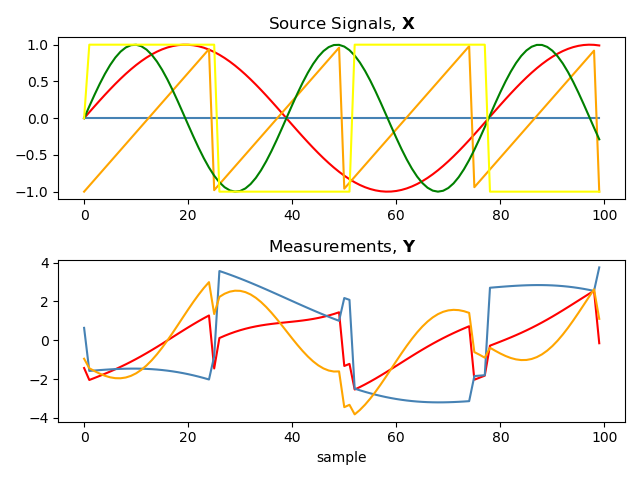
\includegraphics[scale=0.5]{figures/ch_6/simple_data.png}
\caption{Visualization of the signals of the source matrix $\mathbf{X}$ in comparison to the measurement signals of the measurement matrix $\mathbf{Y}$ from the deterministic data set specified by $N = 5, M = 3$, $k = 4$ and $L=1000$.}
\label{fig:simple}
\end{figure}
\noindent

\subsection{Stochastic Data Set}\label{sec:stoch_data}
The purpose of this second kind of data is to resemble EEG measurements for which the model is intended. 
Here different data sets are simulated depending on the chosen specifications of $N$, $k$, $M$ and $L$. 
Every data set is constructed based on four different linear autoregressive processes of various orders, each process representing one source signal:
\begin{itemize}
\item[-] $x_{t}^{1} = \sum_{i=1}^{2} \phi_i x_{t-i}^{1} + w_t^{1}$
\item[-] $x_{t}^{2} = \sum_{i=1}^{2} \zeta_i x_{t-i}^{2} + w_t^{2}$
\item[-] $x_{t}^{3} = \sum_{i=1}^{3} \eta_i x_{t-i}^{3} + w_t^{3}$
\item[-] $x_{t}^{4} = \sum_{i=1}^{4} \xi_i x_{t-i}^{4} + w_t^{4}$
\end{itemize}
where $\boldsymbol{\phi}, \boldsymbol{\zeta}, \boldsymbol{\eta}$ and $\boldsymbol{\xi}$ are different model parameters and $w_t^{j}$ for $j = 1,\dots ,4$ are mutually independent Gaussian distributed white noise sources.
$\mathbf{X}$ is constructed by drawing $k$ autoregressive processes randomly each of length $L$ among the four. If $k < N$ zero rows are inserted randomly such that $\mathbf{X} \in \mathbb{R}^{N \times L}$. 
The mixing matrix $\mathbf{A}$ of size $M \times N$ is, like previously, generated randomly from a Gaussian distribution.
By multiplying the source matrix and the mixing matrix, the measurement matrix $\mathbf{Y}$ is achieved.
The stochastic data set then consist of $\{ \mathbf{Y}, \mathbf{X}, \mathbf{A} \}$. 

One simulation of a stochastic data set is illustrated in figure \ref{fig:AR}. The illustrated data set is specified by $N = 5$, $M = 3$, $k = 4$ and $L = 1000$.
\begin{figure}[H]
\centering
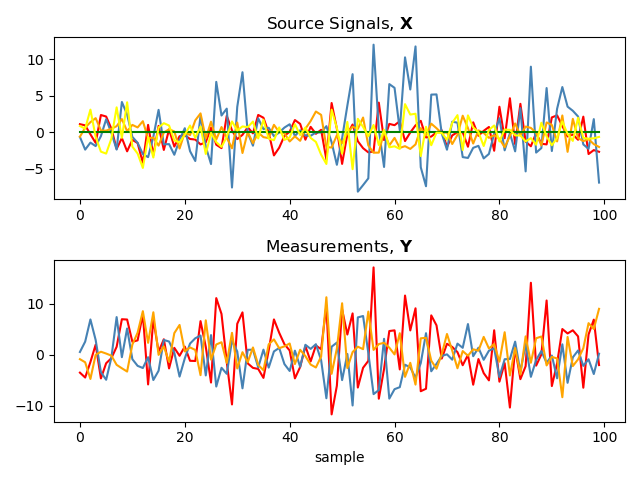
\includegraphics[scale=0.5]{figures/ch_6/AR_data.png}
\caption{Visualization of the source signals of the source matrix $\mathbf{X}$ in comparison to the measurement signals of the measurement matrix $\mathbf{Y}$ from a stochastic data set specified by $N = 5$, $M = 3$, $k = 4$ and $L=1000$. For simplicity only samples [0:100] are plotted.}
\label{fig:AR}
\end{figure}
\noindent

